\documentclass[times, utf8, diplomski]{fer}

\usepackage{booktabs}
\usepackage{float}
\usepackage{algpseudocode}
\usepackage{algorithm}

\algnewcommand{\Or}{\textbf{ or }}
\algnewcommand{\And}{\textbf{ and }}
\newcommand{\classname}[1]{\texttt{#1}}

\graphicspath{ {./images/Transport/} {./images/HLAPI/} }
\setcitestyle{numbers}
\setcitestyle{square}

\begin{document}

\thesisnumber{2963}
\title{Razvoj i primjena biblioteke za umrežavanje višekorisničkih videoigara}
\author{Filip Nemec}
\maketitle

% Ispis stranice s napomenom o umetanju izvornika rada. Uklonite naredbu \izvornik ako želite izbaciti tu stranicu.
% \izvornik

% Dodavanje zahvale ili prazne stranice. Ako ne želite dodati zahvalu, naredbu ostavite radi prazne stranice.
% \zahvala{}

\tableofcontents

\chapter{Transport}
This chapter introduces and explains in detail the concept of a transport layer. It starts by giving an introduction to networking, explaining motivation behind a layered structure. It then discusses today's most widely used transport layers. Finally, it finishes by giving a detailed look into a custom transport layer implementation.

\section{Introduction}
Computer networking is a very complex problem. It consists of many different sub-problems, such as packet-routing, data transmission, integrity, reliability, congestion-control, flow-control and much more. In order to deal with such complexity, ISO (International Organization for Standardization)\footnote{https://en.wikipedia.org/wiki/International\_Organization\_for\_Standardization} developed OSI (Open Systems Interconnection) model\footnote{https://en.wikipedia.org/wiki/OSI\_model} in the year 1984. OSI model divides complex problem of computer networking into a structure consisting of 7 layers\footnote{https://www.geeksforgeeks.org/layers-of-osi-model/}, each layer building on top of the layer below it. Layers are defined as follows:

\begin{enumerate}
	\item \textbf{Physical layer} is responsible for transmission of raw signals between two or more physical entities. Jobs of this layer include transmission of bits, bit-rate control and support for various modes of transmission such as simplex, half-duplex and full-duplex.
	
	\item \textbf{Data-link layer} enables communication between two neighboring network nodes (devices). Basic functions of this layer include point-to-point frame transmission, error-control and data-flow control. 
	
	\item \textbf{Network layer} solves the problem of end-to-end device communication. Functions of network layer include routing (finding optimal route for data to reach its destination) and logical addressing (ability to uniquely identify a device on the computer network).
	
	\item \textbf{Transport layer} is responsible for transmission of data from process-to-process while satisfying transparency criterion. There are two types of transparencies \cite{kommre}:
	
	\begin{enumerate}
		\item \textit{Semantic transparency} whose only task it to ensure that data arrives reliably and in-order it was sent.
		\item \textit{Temporal transparency} that only focuses on delivering data as fast as possible.
	\end{enumerate}

	\item \textbf{Session layer} is responsible for establishing, maintaining and terminating connections, authentication and security.
	
	\item \textbf{Presentation layer} is responsible for encryption/decryption, compression and translation between data formats.
	
	\item \textbf{Application layer} is where all of the data is produced, processed and shown to the end-user. 
\end{enumerate}

With such layered structure, we introduced concept of \textit{abstraction}. Every layer simply uses implementation below it without the need to know how it is implemented. This gives us the ability to easily swap out implementations of different layers in the stack.


\begin{figure}[h!]
	\centering
	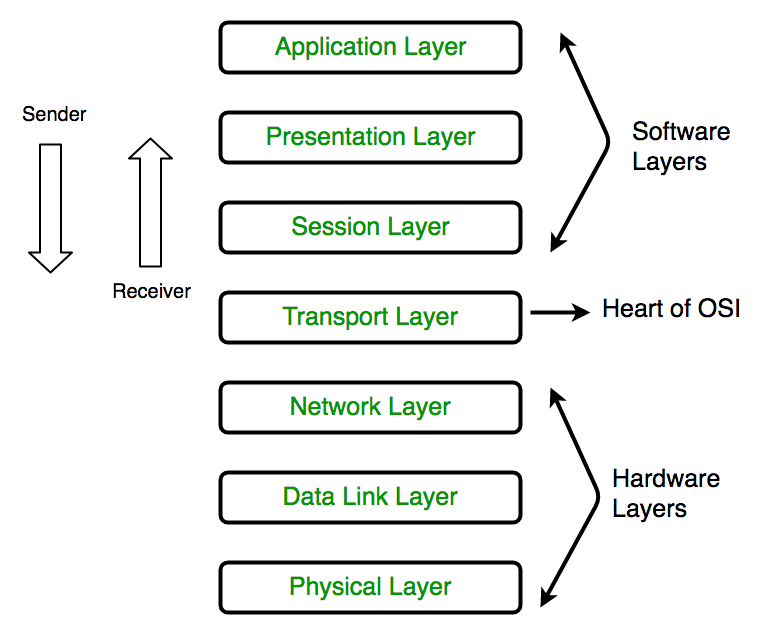
\includegraphics[scale=0.32]{OSI-model-layers}
	\caption{OSI layers, from \cite{GeeksForGeeks:OSI-model}}
\end{figure}


\section{Existing transport implementations}
Previous section mentioned the terms of semantic and temporal transparency. Consequently, there exist two different transport layer implementations, one for each transparency type. \\

The first protocol, which implements semantic transparency, is called TCP (Transmission Control Protocol)\footnote{https://datatracker.ietf.org/doc/html/rfc793}. TCP abstracts away the concept of computer network and exposes a simple interface to the user, where writing bytes is almost the same as writing to a simple binary file. \\

The second protocol, which implements temporal transparency, is called UDP (User Datagram Protocol)\footnote{https://datatracker.ietf.org/doc/html/rfc768}. UDP is a protocol that implements a thin layer of abstraction over the network layer.

\begin{figure}[h!]
	\centering
	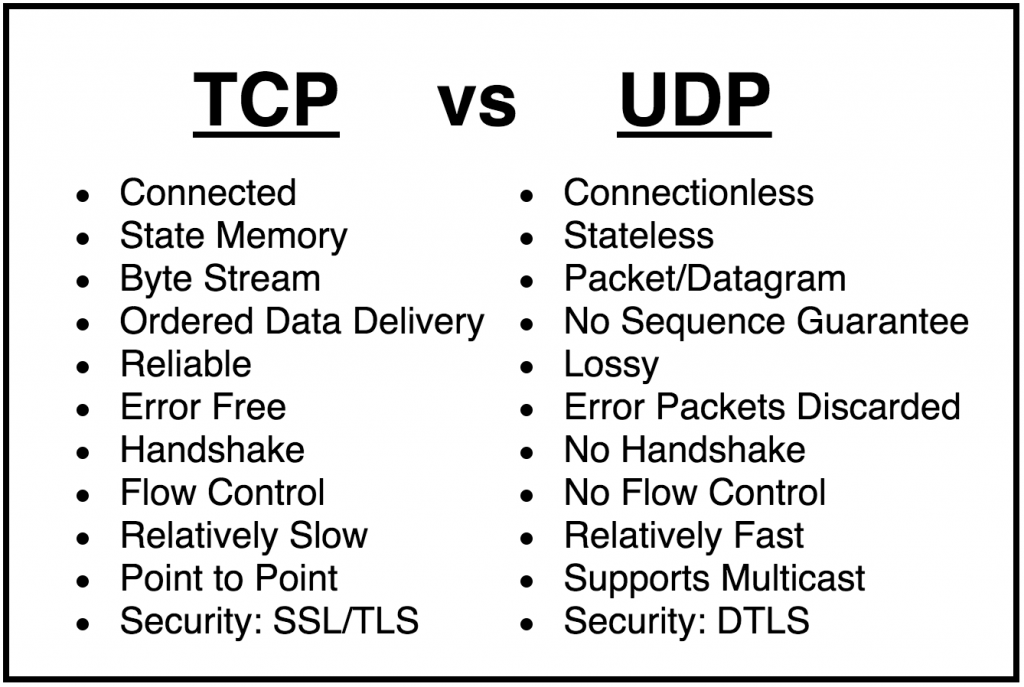
\includegraphics[scale=0.5]{TCP-vs-UDP}
	\caption{Comparison between TCP and UDP protocols, from \cite{NetBurner:TCP-vs-UDP}}
\end{figure}


\section{Custom transport implementation}
While TCP and UDP are great at solving their own use-cases, there exists a major problem: each protocol solves only one type of transparency. With the rise of online gaming, there appeared the need for having both transparency implementations at once; some data would require reliability and ordering that TCP provides (for example, textual chat messages), while other types needed only latest data without the guarantee of delivery (for example, position of the player in a virtual world). \\

Using both protocols at the same time, based on the type of data, is not an ideal solution either, for multiple reasons \cite{GafferOnGames:UDP-vs-TCP}:

\begin{enumerate}
	\item Using TCP can induce packet loss in UDP packets as routers often prioritize TCP segments (as dropping TCP segment requires re-sending, while dropping UDP packet does not).
	\item Supporting many reliable channels (for example, one channel for text message data, another for images or audio) would require many TCP connections, quickly exhausting operating system resources.
	\item Application code-base would be hard to manage, potentially resulting in slower development and harder to track bugs.
\end{enumerate}

For all of those reasons, a custom solution is required - one that allows the user to easily specify, on per packet basis, how data should be delivered. If data is time-sensitive, user must be able to send it in unreliable manner, where temporal transparency is preserved. If data is important and must be delivered, semantic transparency must be preserved. As UDP already provides temporal transparency, we simply need to upgrade it with optional semantic transparency features that are present in the TCP. Implementations of such protocols are often called RUDP - \textit{Reliable User Datagram Protocol}. The rest of this chapter explains one such implementation.



\subsection{Packet}
\classname{Packet} represents a single outgoing message of arbitrary data that can be sent over the network. It is a thin abstraction layer over raw byte-array and therefore offers some of the benefits that a raw byte-array cannot. \\

One such benefit is object pooling\footnote{https://en.wikipedia.org/wiki/Object\_pool\_pattern}. As creation of packets is a very frequent occurrence in networked applications, allocating new packet instances (which also internally keeps a medium sized byte-array) each time a packet is needed would quickly fill-up heap memory, prompting execution of garbage collection\footnote{https://en.wikipedia.org/wiki/Garbage\_collection\_(computer\_science)}. This is especially important in applications that have time constraints, such as games, where even one slowly executed frame could ruin user experience. \\

Another benefit is separation of write-only and read-only operations. Since \classname{Packet} represents an outgoing packet, it only offers methods for writing data (constructing the packet). Those methods also provide powerful functionality, allowing user to construct packets containing complex structures. \\

\begin{figure}[h!]
	\centering
	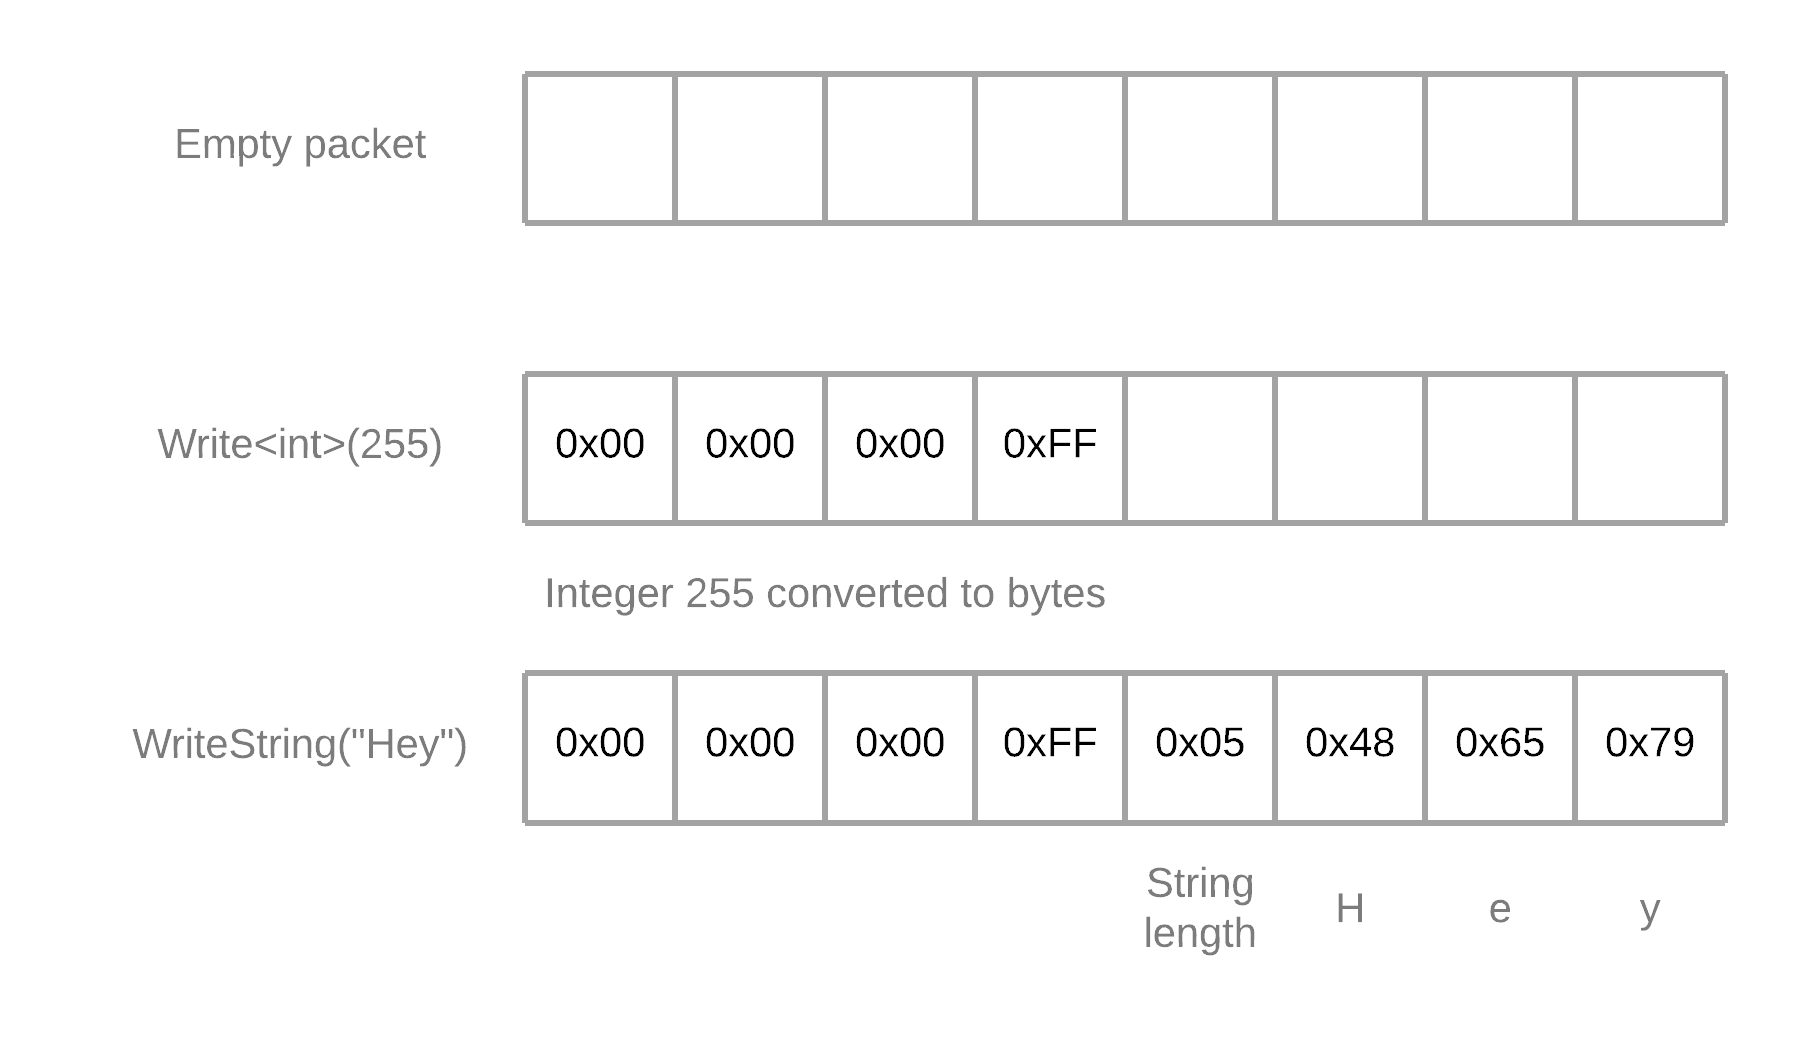
\includegraphics[scale=0.22]{Packet-write}
	\caption{Example of writing data to a packet}
\end{figure}

Similarly to \classname{Packet}, which is write-only, there exists a read-only packet version named \classname{Read\-Only\-Packet} which represents a single incoming message of arbitrary data that was received over the network. It offers the same interface as \classname{Packet}, but instead of write, read methods are exposed. Another important feature of \classname{Read\-Only\-Packet} is that it cannot in any way modify underlying packet data, making it very safe to use, even in multi-threaded scenarios. \\

Finally, the last benefit is cleaner code. Spotting an instance of \classname{Packet} or \classname{Read\-Only\-Packet} immediately gives information to the reader that this code works with networking. Same could not be said for byte-array as its usages are much broader. \\

\classname{Packet} also defines an important constant, which is the maximum size, in bytes. This constant is carefully chosen to avoid packet fragmentation on the network layer. Any packets that require bigger size must use a fragmented channel which will perform fragmentation and reassembly on the application layer. Maximum size is equal to Ethernet MTU (Maximum transmission unit, 1500 bytes) subtracted by IP header size (20 bytes) and UDP header size (8 bytes), which results in maximum size of 1472 bytes.\\

\begin{equation}
	Maximum \; size = 1500 - 20 - 8 = 1472 \; bytes \label{eq:max_packet_size}
\end{equation}

\subsubsection{Packet structure}
Each packet follows the same structure, which is a header type followed by the header-specific payload. It is important to mention that header is always inserted as the first byte without any exceptions.

\begin{figure}[h!]
	\centering
	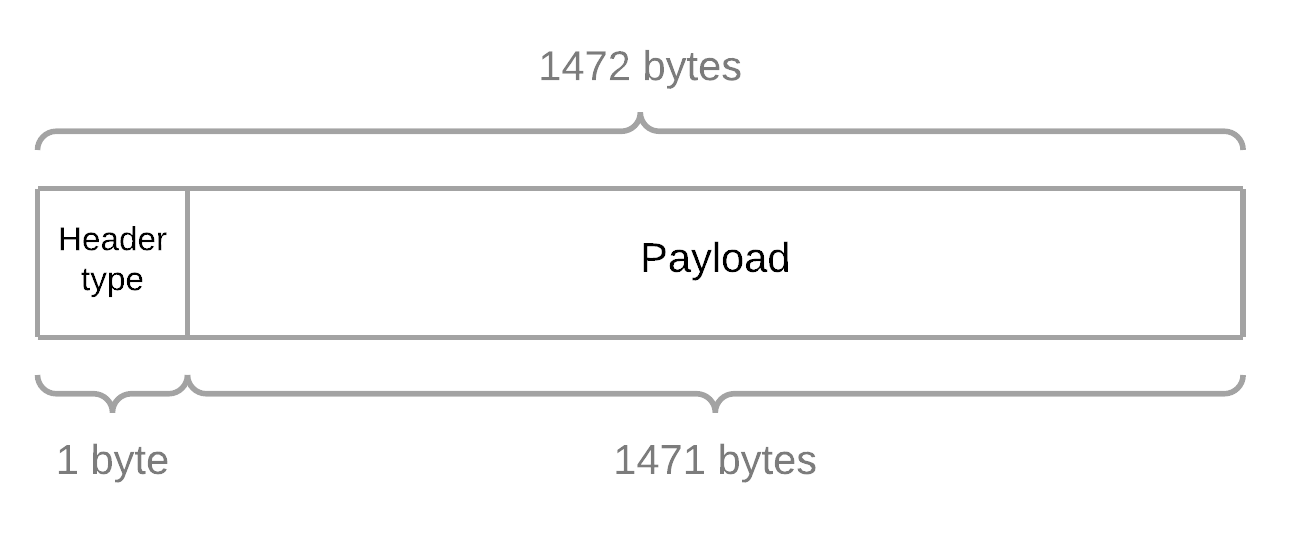
\includegraphics[scale=0.25]{Packet-structure}
	\caption{Packet structure}
\end{figure}


\subsubsection{Header types}
Header type is used to denote what kind of packet it is and allows the receiver to decode the meaning behind received bytes.

\begin{table}[H]
	\centering
	\resizebox{\textwidth}{!}{%
		\begin{tabular}{|c|c|c|}
			\hline
			\textbf{Header type} & \textbf{Description}                                                                                                                   & \textbf{Payload}                                                                       \\ \hline
			Connect              & \begin{tabular}[c]{@{}c@{}}Sent by the client to server when\\ establishing a virtual connection.\end{tabular}                         & Optional connect data                                                                  \\ \hline
			ConnectApproved      & \begin{tabular}[c]{@{}c@{}}Sent by the server to client when\\ connection request has been approved.\end{tabular}                      & -                                                                                      \\ \hline
			Ping                 & \begin{tabular}[c]{@{}c@{}}Used for measuring connection latency\\ and serves as a keep-alive packet.\end{tabular}                     & Sequence number                                                                        \\ \hline
			Pong                 & Response to the ping packet.                                                                                                           & Sequence number                                                                        \\ \hline
			Data                 & Indicates that the packet contains data.                                                                                               & \begin{tabular}[c]{@{}c@{}}Channel ID, channel header,\\ application data\end{tabular} \\ \hline
			Acknowledgement      & \begin{tabular}[c]{@{}c@{}}Indicates that specific set of\\ packets have been received.\end{tabular}                                   & \begin{tabular}[c]{@{}c@{}}Channel ID, sequence number,\\ ack bit-field\end{tabular}   \\ \hline
			Disconnect           & \begin{tabular}[c]{@{}c@{}}Sender has closed its side of the connection and\\ will no longer send or receive any packets.\end{tabular} & -                                                                                      \\ \hline
			Timeout              & Indicates that a connection has timed-out.                                                                                             & -                                                                                      \\ \hline
		\end{tabular}%
	}

	\caption{All of the possible header types.}
	\label{table:header-types}
\end{table}

Only one header type is special, and that is the \textit{Data} type, as that is the only type with which the end-user is going to interact with.

\begin{figure}[h!]
	\centering
	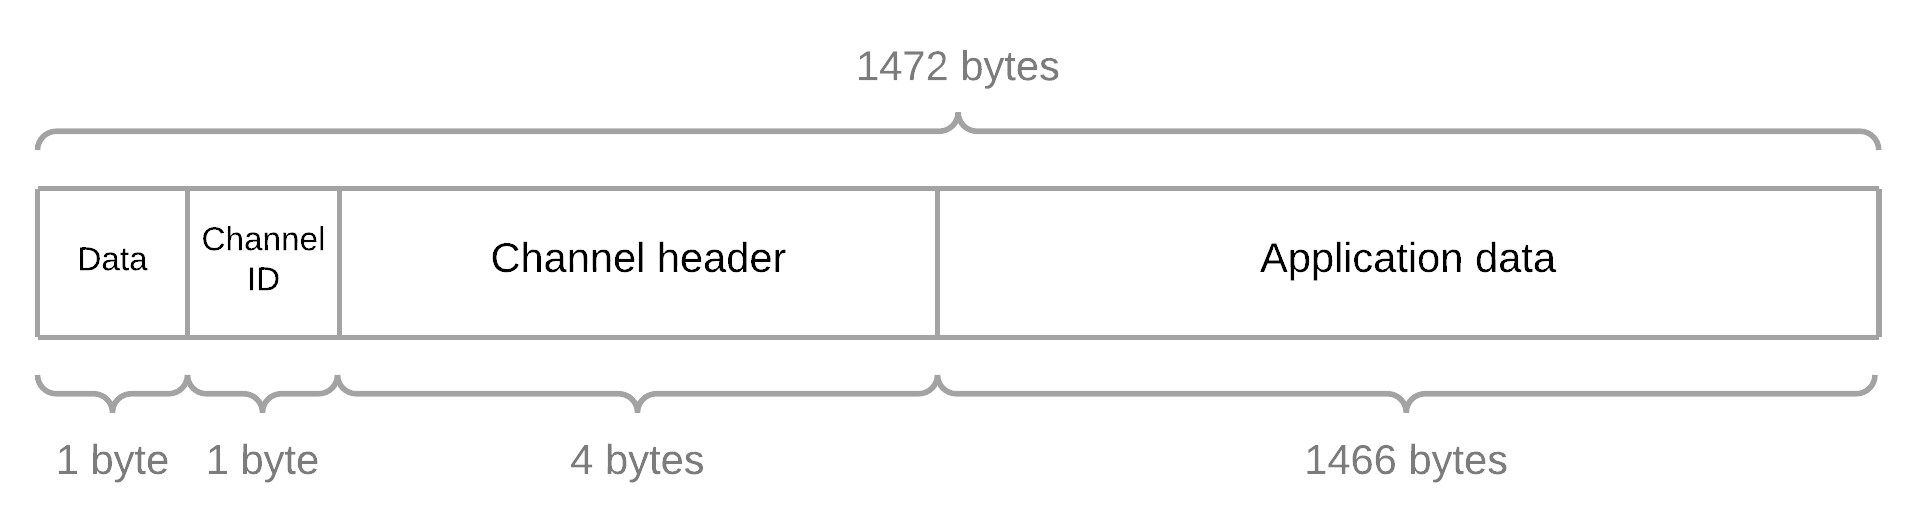
\includegraphics[scale=0.2]{Data-packet-structure}
	\caption{Data-packet structure}
\end{figure}


\subsection{Array pooling}
Fluid gameplay with no stuttering is essential for user experience. Standard value that always needs to be maintained is at least 60 frames per second\footnote{https://en.wikipedia.org/wiki/Frame\_rate} (FPS). Failing to render at least that many frames each second is going to result in noticeable lag, drastically decreasing overall user satisfaction. This constraint means that all of the updates need to be performed in about 16 milliseconds. Consequently, this implies that expensive, long-running operations should be run as rarely as possible. One such operation is the process of garbage collection\footnote{https://en.wikipedia.org/wiki/Garbage\_collection\_(computer\_science)}, where all of the previously allocated memory that is no longer referenced is being freed.\\

However, garbage collection is only triggered when memory is no longer referenced. If we keep a reference to previously allocated memory and reuse it, no garbage collection will be performed. Such process of reusing memory is called \textit{object pooling}\footnote{https://en.wikipedia.org/wiki/Object\_pool\_pattern} and is a standard practice in high-performance applications. As networked applications constantly keep sending packets back and forth (and packets are essentially just arrays of bytes), utilizing object pooling is perfectly suitable.\\

In our implementation, array pooling is implemented using an array of buckets. In this context, term \textit{bucket} means a collection of reusable arrays. Each bucket holds multiple arrays of same sizes and each subsequent bucket holds arrays of exponentially increasing capacities. First bucket holds arrays of size \textit{Packet.MaxSize}. Last bucket holds arrays of sizes \textit{Packet.MaxSize * 256}, which is maximum allowed size of a fragmented packet.


\begin{figure}[h!]
	\centering
	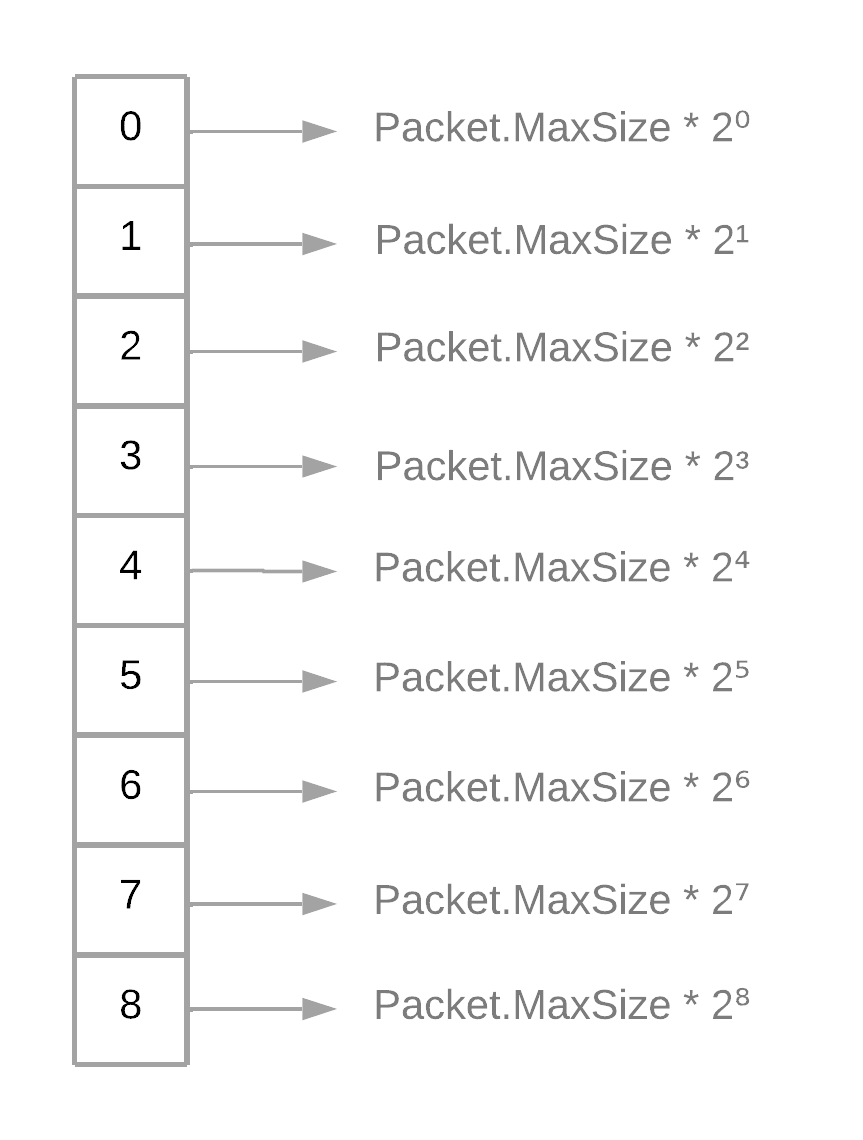
\includegraphics[scale=0.2]{Array-pool-buckets}
	\caption{Array pool buckets}
\end{figure}



\subsection{Channels}
Channel represents a component that controls the way packets are sent and received. There are four fundamental problems that a channel can, but does not have to solve:

\begin{enumerate}
	\item \textbf{Order} - ability for the receiver to receive packets in order in which they were originally sent.
	\item \textbf{Duplication} - ability for receiver to detect and discard duplicate packets.
	\item \textbf{Reliability} - ability for sender to ensure that receiver received a packet.
	\item \textbf{Fragmentation} - ability for sender to divide a big packet into smaller packets called \textit{fragments} and for receiver to reassemble those into original big packet.
\end{enumerate}

\begin{center}
	\begin{table}[H]
		\centering
		
		\begin{tabular}{ |c|c|c|c|c|c| } 
			\hline
			Name & Order & Duplication & Reliability & Fragmentation \\ 
			\hline
			Unreliable        & - & - & - & - \\ 
			Sequenced         & Yes & Yes & - & - \\ 
			Reliable          & Yes & Yes & Yes & Yes \\ 
			\hline
		\end{tabular}
		
		\caption{Channel implementations and problems each implementation solves}
	\end{table}
\end{center}

Each channel also has a name associated with it and keeps track of bandwidth statistics, which is useful for diagnosing network usage. Information tracked by the channel are following state variables:

\begin{enumerate}
	\item \textbf{Packets sent} represents total number of packets sent through the channel.
	\item \textbf{Bytes sent} represents total number of bytes sent through the channel.
	\item \textbf{Packets received} represents total number of packets received on the channel.
	\item \textbf{Bytes received} represents total number of bytes received on the channel.
\end{enumerate}



\subsubsection{Unreliable channel}
Unreliable channel is the most basic channel type that does no processing of sent and received packets. Since it does not perform any logic, this channel type does not use any header bytes in the packet. It acts as a pure UDP socket, therefore it does not provide any insurance:

\begin{enumerate}
	\item Packets can arrive out-of-order and receiver has no way of reassembling packets in order.
	\item Packets can be duplicated in the network and receiver has no way of knowing it received a duplicate packet.
	\item Packets can be lost in the network and sender has no way of knowing if packet was potentially lost in transit.
	\item Packet size is limited as there is no support for fragmentation and reassembly.
\end{enumerate}

\begin{figure}[h!]
	\centering
	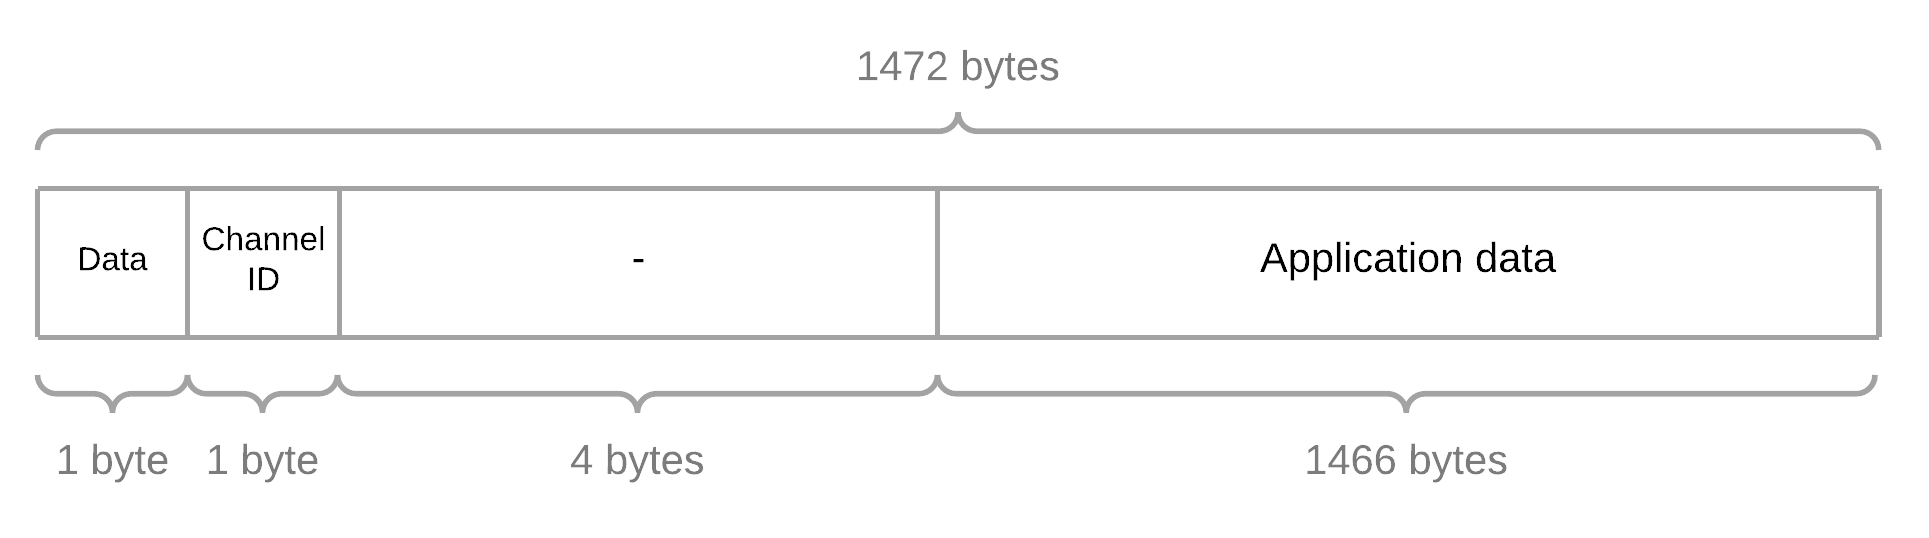
\includegraphics[scale=0.2]{Unreliable-packet-structure}
	\caption{Format of the packet sent through the unreliable channel.}
\end{figure}



\subsubsection{Sequenced channel}
Sequenced channel solves two problems: order and duplication. It does so by attaching a unique number to each outgoing packet called \textit{local sequence number}, which is a state variable maintained by the sending side of the channel. For each packet sent, local sequence number is incremented.

\begin{figure}[h!]
	\centering
	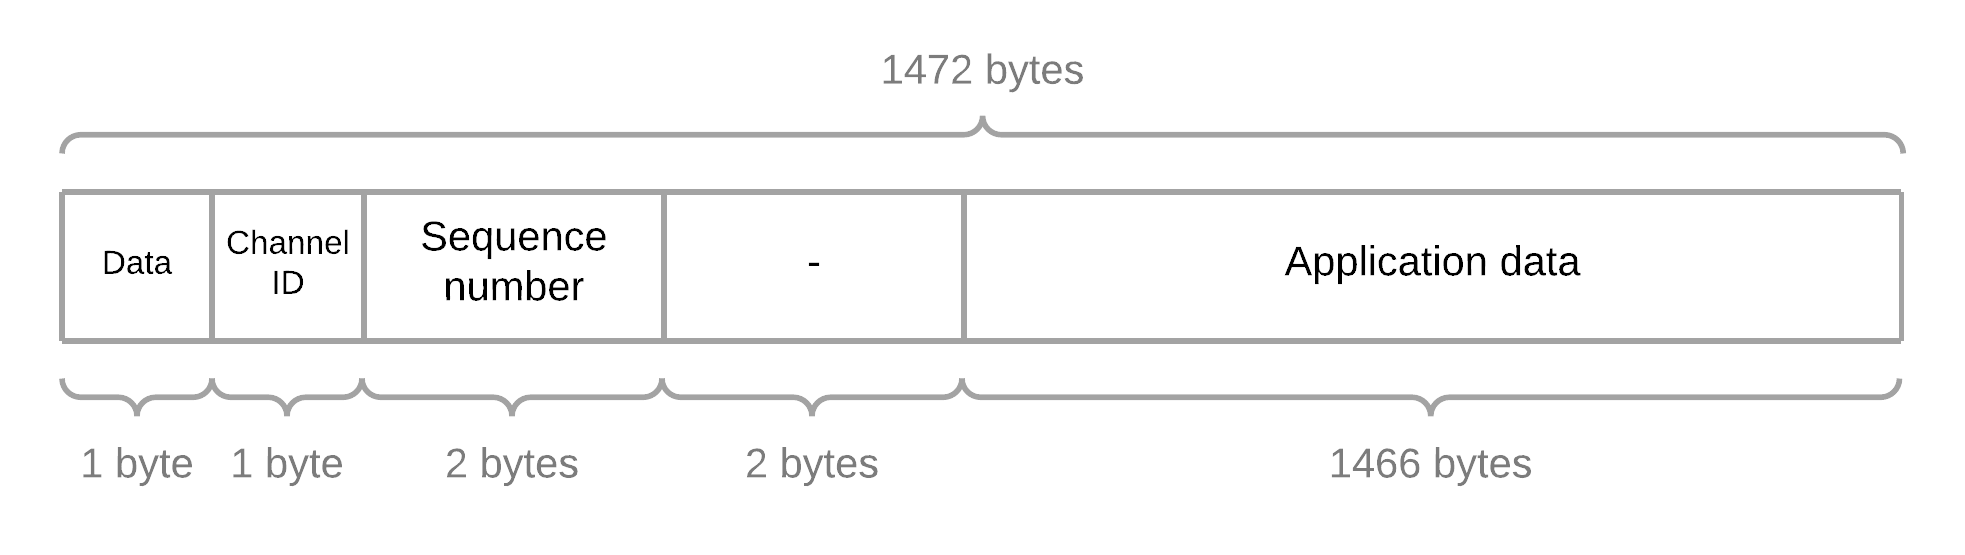
\includegraphics[scale=0.2]{Sequenced-packet-structure}
	\caption{Format of the packet sent through the sequenced channel.}
\end{figure}

On the receiver side, another state variable is maintained: \textit{remote sequence number}. The remote sequence number holds the value of the highest received sequence number and this value is used to determine whether a newly received packet should be accepted or discarded. \\

Once a new packet is received, the sequence number is read from the packet. If the sequence number contained in the packet is greater than the remote sequence number, packet is accepted, otherwise it is discarded. \\

Another problem needs to be addressed: sequence number wrapping. As sequence numbers are stored in only 2 bytes, maximum sequence number value can be 65535. Once this sequence number is reached, next packet sequence number is going to wrap back to the minimum value of 0. Using naive approach of comparing raw sequence number values is going to produce wrong results; even though 65535 is numerically greater than 0, it logically is not. To solve this problem, the following algorithm is used to compare sequence numbers:

\begin{algorithm}[H]
	\caption{Comparing sequence numbers with wrapping}
	\textbf{Input:} First sequence number $seq1$, second sequence number $seq2$ \\
	\textbf{Output:} $true$ if $seq1$ is greater than $seq2$, $false$ otherwise \\
	
	\begin{algorithmic}
		\State $isGreaterRegular \gets seq1 > seq2 \And seq1 - seq2 \leq 32767$
		\State $isGreaterWithWrap \gets seq1 < seq2 \And seq2 - seq1 > 32767$ \\
		\Return $isGreaterRegular \Or isGreaterWithWrap$
	\end{algorithmic}
\end{algorithm}

Algorithm is based on a simple idea: if sequence number values are close numerically, wrapping did not occur. Sequence numbers are close if absolute value of their difference is smaller or equal to half of the full sequence number range.


\subsubsection{Reliable channel}
Reliable channel solves all four problems: order, duplication, reliability and fragmentation. The rest of this section is going to cover in detail how reliability and fragmentation were solved.\\

To solve reliability, packet acknowledgments and re-transmission concepts are borrowed from TCP. The idea is that each packet sent needs to be acknowledged by the receiver. If packet is not acknowledged in a certain amount of time, it is considered lost and will be re-transmitted. A packet that has been sent, but not yet acknowledged by the receiver is called a \textit{pending packet}. \\

Each pending packet internally maintains a timer that will, if expired, automatically resend the packet. If acknowledgment is received before timer expires, timer is canceled and pending packet is removed from the collection of active pending packets. To prevent sending packets \textit{ad infinitum}, each pending packet internally counts number of re-transmission attempts. If the counter exceeds maximum number of attempts (value which is defined by the channel), connection is deemed lost and will be timed-out. \\

\begin{figure}[H]
	\centering
	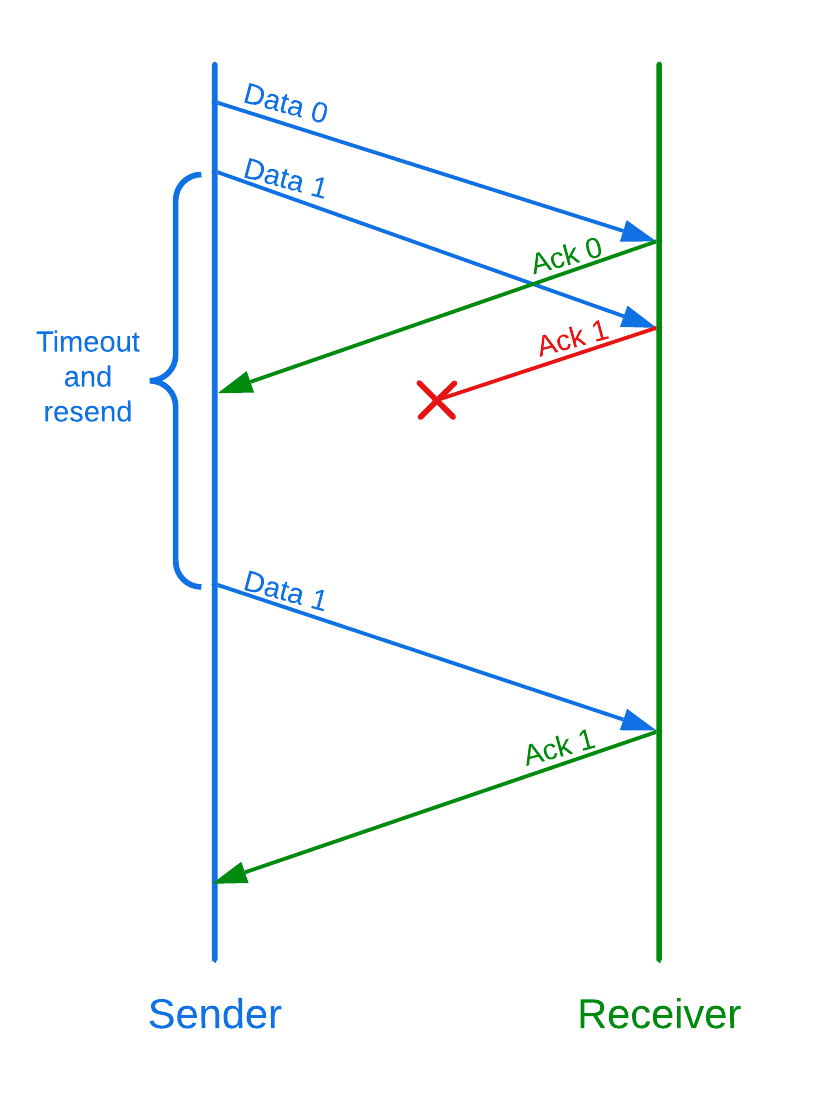
\includegraphics[scale=0.3]{Resend-diagram}
	\caption{Resend diagram that shows how data and acknowledgment packets are sent and received. Diagram shows that data-packet 0 was successfully acknowledged and did not require a resend. Meanwhile, acknowledgment of data-packet 1 was lost in transit, which in turn made sender's timer time-out, causing data-packet 1 to be resent.}
\end{figure}

On the receiving side of the channel, array of received packets is maintained. It is an array that is updated in the following manner: for each received packet, sequence number is read from the header. If array slot at index which is equal to sequence number is empty, that means received packet is not a duplicate and is stored in the array. If the slot is already filled, that means received packet is a duplicate and is discarded. If a packet was successfully stored, acknowledgment is sent to the sender. \\

Acknowledgment packet has the ability to acknowledge multiple packets at once. Naive approach would be to simply send an array of several most recently received packet sequence numbers. However, since each sequence number is a 16-bit integer, that approach is very bandwidth inefficient. Much more efficient approach is to use so called \textit{anchor sequence number} combined with additional acknowledgment bit-field. \\

Anchor sequence number is an actual 16-bit sequence number and it is equal to the sequence number of the most recently received packet. Acknowledgment bit-field is a bit-field in which each bit is responsible for acknowledging a sequence number relative to anchor. Concretely, first bit is responsible for indicating whether packet with sequence number \textit{anchor - 1} has been received. If bit is set, it means packet was received, otherwise it wasn't. In general, bit at position \textit{n} is responsible for indicating whether packet with sequence number \textit{anchor sequence number - n} has been received. With this approach, 8 previous sequence numbers can be acknowledged using only 1 additional byte of data. This approach achieves perfect entropy\footnote{https://en.wikipedia.org/wiki/Entropy\_(information\_theory)}.\\

\begin{figure}[H]
	\centering
	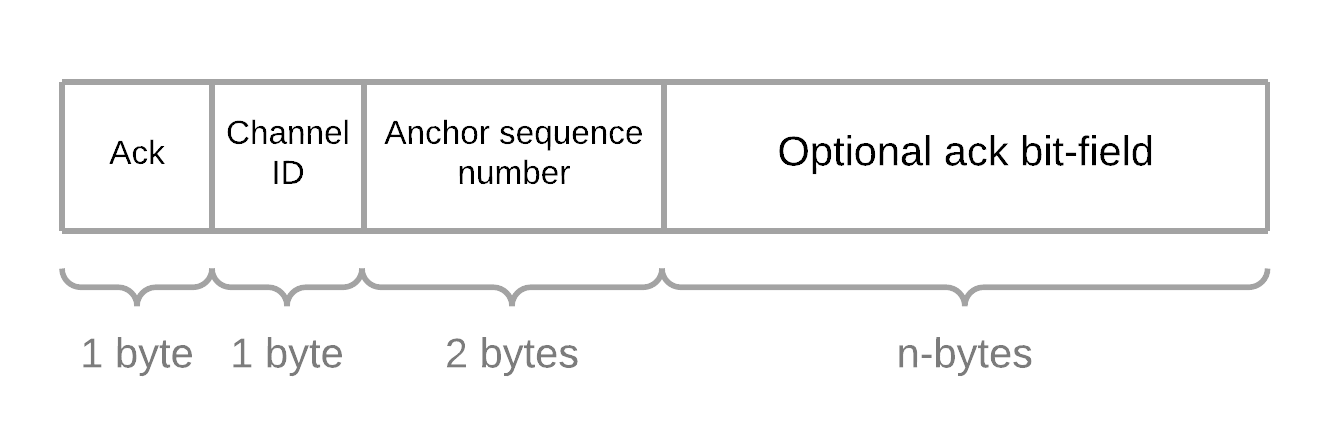
\includegraphics[scale=0.25]{Ack-packet-structure}
	\caption{Format of the acknowledgment packet sent through the reliable channel.}
\end{figure}

In order for receiver to receive packets in actual order they were originally sent, another state variable is used: \textit{receive sequence number}. It represents the next expected packet sequence number. Once a packet with that sequence number is received, packet is forwarded to the library user and receive sequence number is incremented. If packet is received out-of-order (for example, packet with number 7 is received before 6), packet is buffered for later.

\begin{figure}[H]
	\centering
	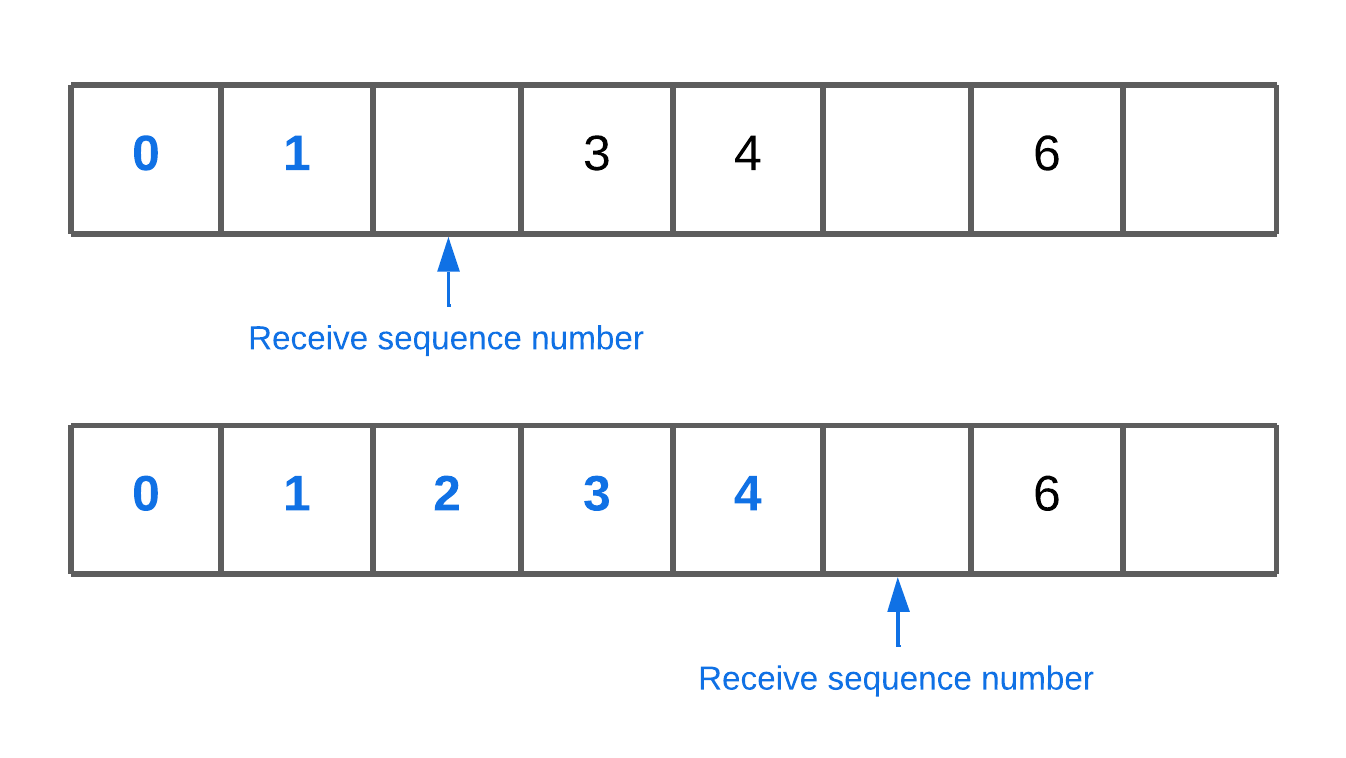
\includegraphics[scale=0.25]{Ordered-receive}
	\caption{Ordered receive implemented using \textit{receive sequence number}. Array slots that have numbers in it represent already received and stored packets, while empty slots are packets that haven't been received yet. Blue numbers represent packets that have been forwarded to library user. First array shows that sequence number 2 is expected and that packets 3, 4 and 6 have been already received, but haven't been forwarded to the user (as forwarding would violate order since packet 2 still hasn't been received). Second array shows what happens when packet 2 is received. Packet 2 is forwarded, but also 3 and 4 since those packets have been received earlier. At the end of it, next expected sequence number is 5.}
\end{figure}

With the previously described system packets are always received in-order and are guaranteed to be delivered (or connection times-out if maximum number of resend attempts are exceeded). This channel property allows implementation of another very useful feature: fragmentation and reassembly of big packets \cite{GafferOnGames:Sending-large-blocks-of-data}.\\

Fragmentation is a process of breaking up a big packet into multiple smaller packets called \textit{fragments} which can be easily transferred over the network. A big packet is defined as a packet whose size exceeds maximum packet size \eqref{eq:max_packet_size}. Fragmentation is performed by the sending side of the channel. Reassembly is the reverse process: combining fragments into the original big packet. Reassembly is performed by the receiving side of the channel. \\

\begin{figure}[H]
	\centering
	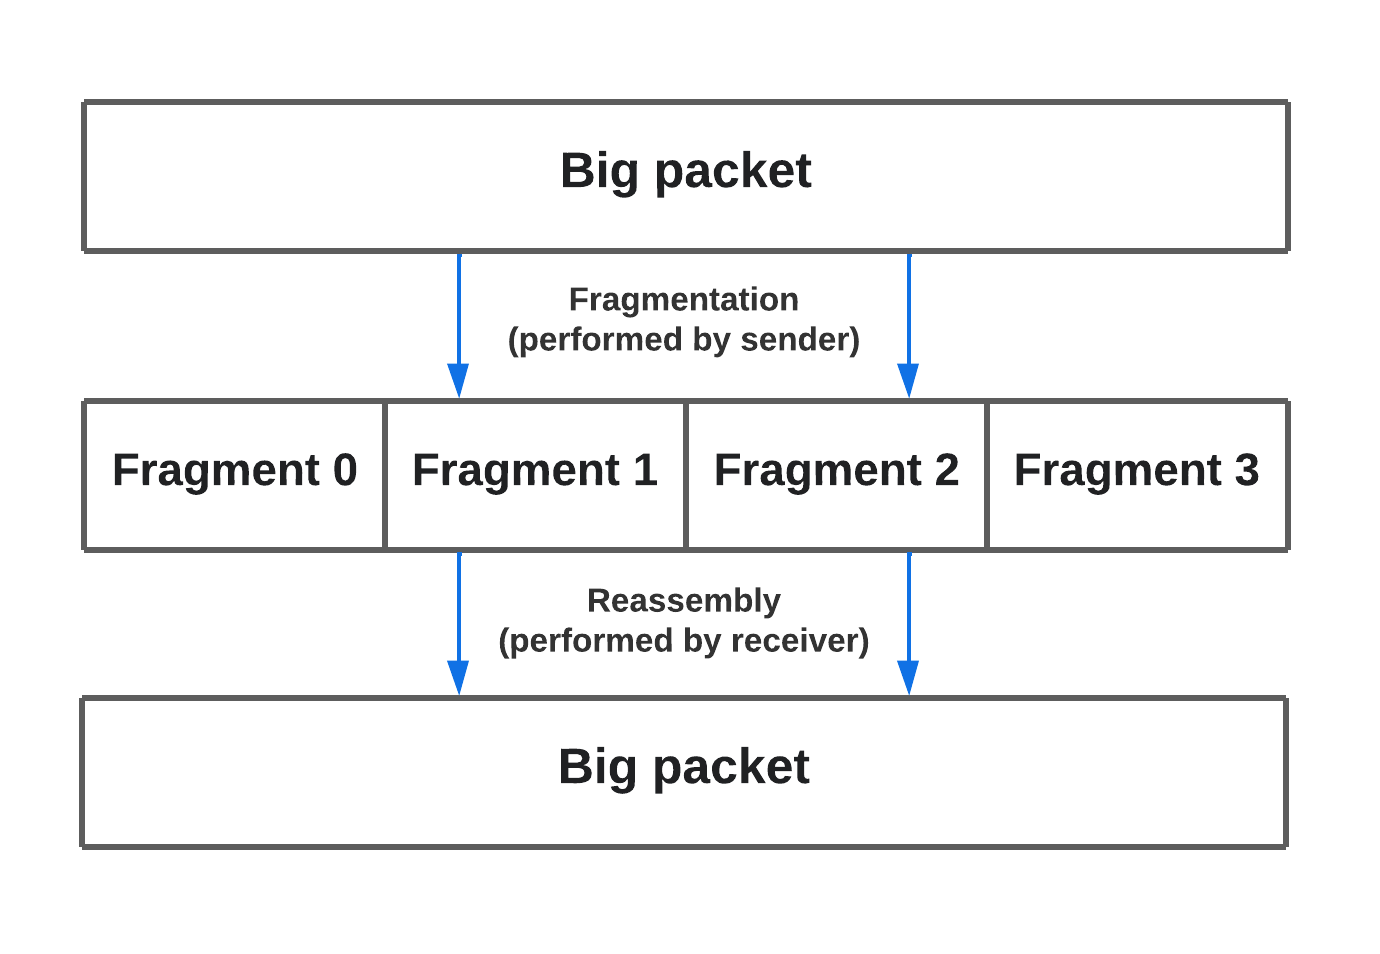
\includegraphics[scale=0.3]{Fragmentation-and-reassembly}
	\caption{Simple flow diagram of fragmentation and reassembly.}
\end{figure}

In order to support fragmentation and reassembly, additional fields need to be attached to each packet. First field is \textit{fragment index} which defines a position in the original big packet. Second field is \textit{fragment count} that states how many fragments a big packet consists of.

\begin{figure}[H]
	\centering
	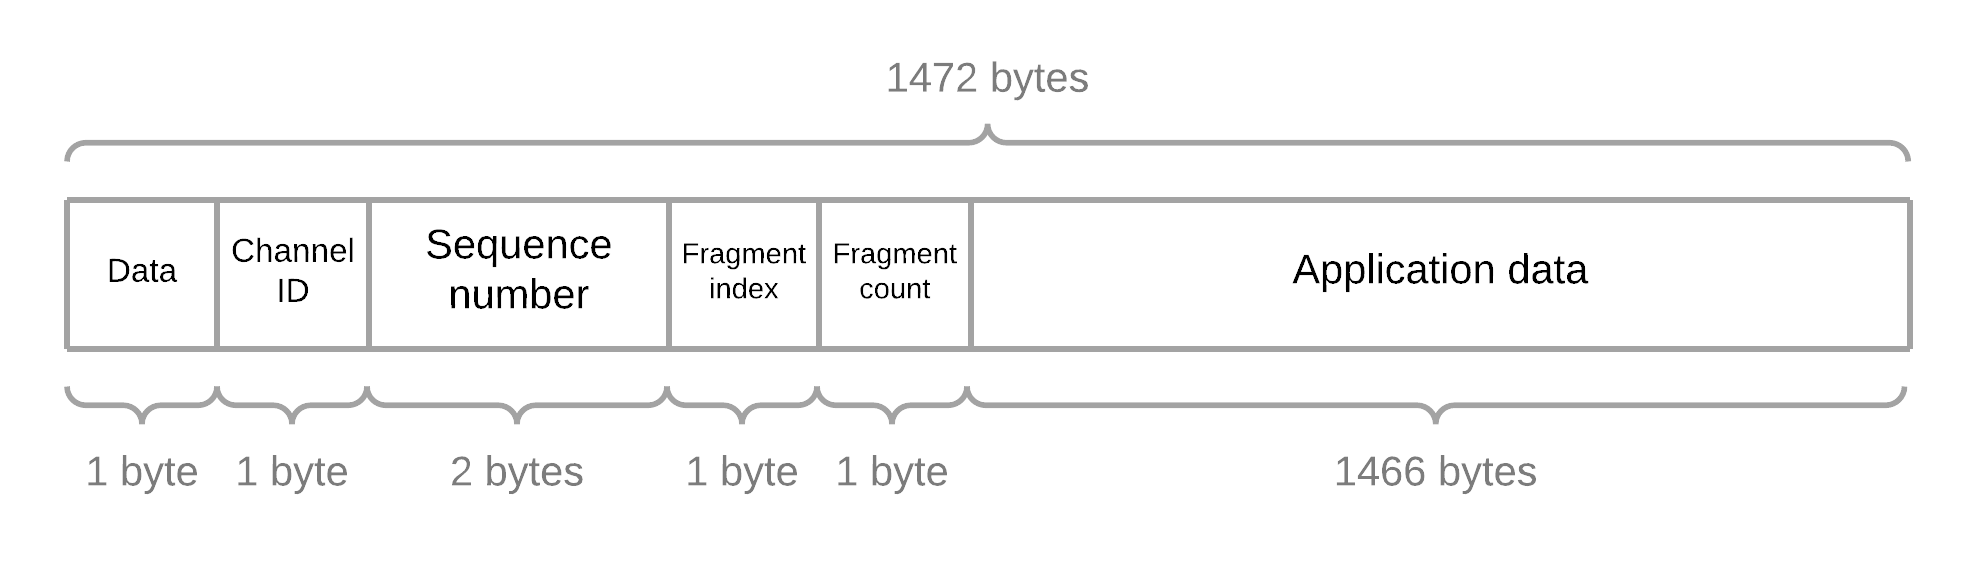
\includegraphics[scale=0.2]{Reliable-packet-structure}
	\caption{Format of the packet sent through the reliable channel.}
\end{figure}

Fragmentation on the sender side of the channel is performed as follows: each time a packet is being sent, total number of fragments required is calculated (based on the packet size). If packet consists of only a single fragment, that means fragmentation is not needed and packet is sent as is (with fragment index set to 0 and fragment count set to 1). If packet consists of multiple fragments, big packet's payload is distributed into multiple fragments (each storing only a fraction of the big packet) and then each fragment is sent. \\

Reassembly on the receiver side of the channel is performed as follows: if a fragment with count of 1 is received, it is immediately forwarded to the user. If fragment count is greater than 1, receiver attempts to reassemble original big packet. It can only do so if all of the fragments have been received.

\begin{figure}[H]
	\centering
	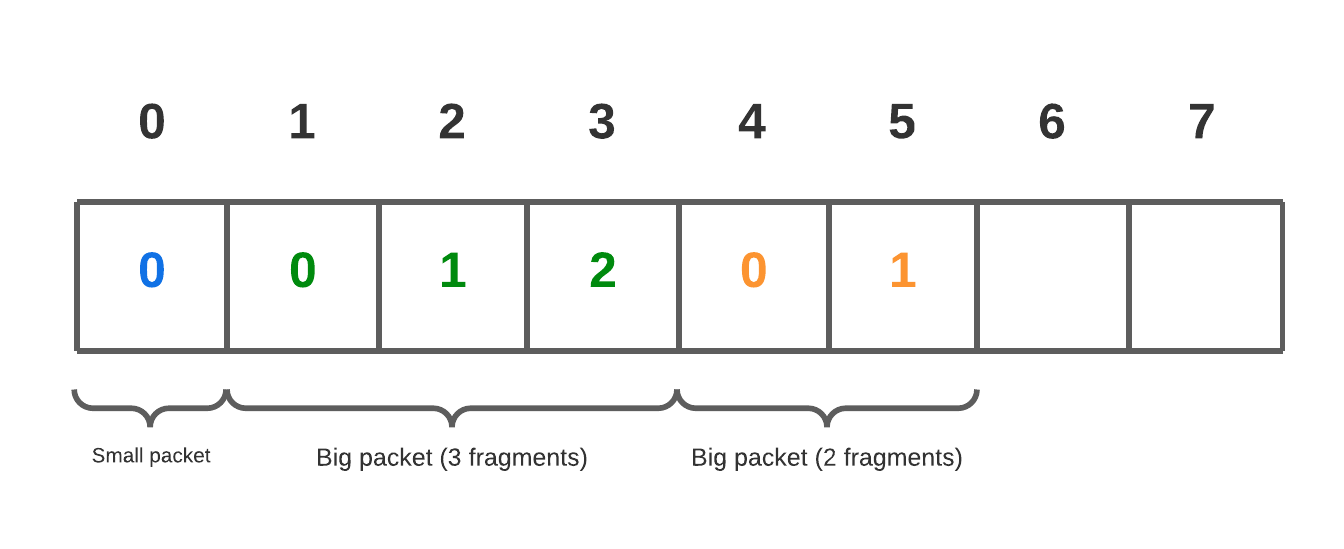
\includegraphics[scale=0.3]{Fragmentation-pending-packets}
	\caption{Example of received packets array combined with fragmentation and reassembly system. Numbers above the array represent packet sequence numbers. Numbers in the array slots represent fragment indexes. Numbers with the same color belong to the same original big packet. Once receiver receives all of the required fragments (which it can deduce based on the fragment count attached to each fragment), it can reassemble original big packet. }
\end{figure}

This fragmentation and reassembly implementation allows users to efficiently and safely send packets with sizes up to $1466 \times 255 = 373830 \; bytes$.



\subsection{Connection}
Connection represents a link between two network nodes. It is a higher level component that has multiple responsibilities:

\begin{enumerate}
	\item Holds an array of channels and is responsible for forwarding packets to the corresponding channel.
	\item Calculates round-trip time by sending ping packets and automatically performs time-out if no valid response is received in certain amount of time.
	\item Keeps track of bandwidth statistics (total number of packets/bytes that were sent/received).
\end{enumerate}

Each connection can have up-to 256 channels. Channels are differentiated by their ID, which is a single byte value.

\begin{figure}[H]
	\centering
	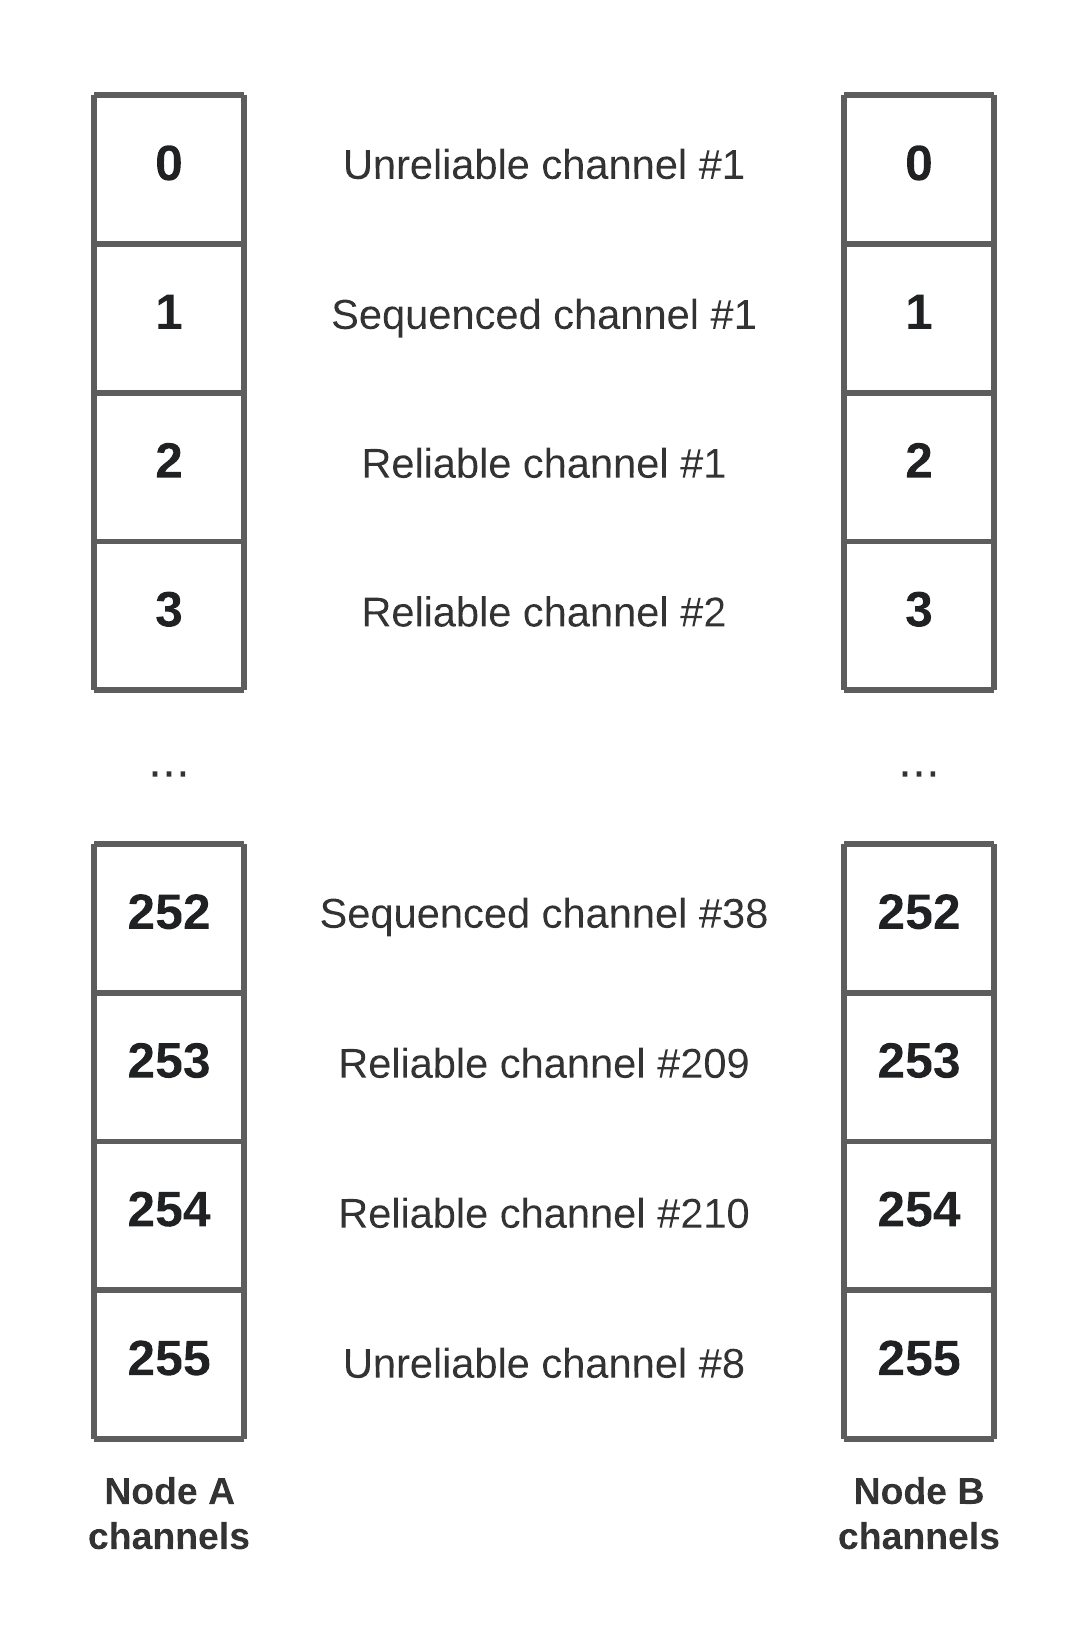
\includegraphics[scale=0.2]{Connection-channels}
	\caption{Example of channel array that is maintained by the connection.}
\end{figure}



\subsection{Nodes}
Final piece of the puzzle is an actual network node. A network node represents a fundamental building block of any network graph that can send and receive data. A graph\footnote{https://en.wikipedia.org/wiki/Graph\_theory\#Graph} consists of vertices (which are represented by nodes) and edges (which are represented by connections).

\begin{figure}[H]
	\centering
	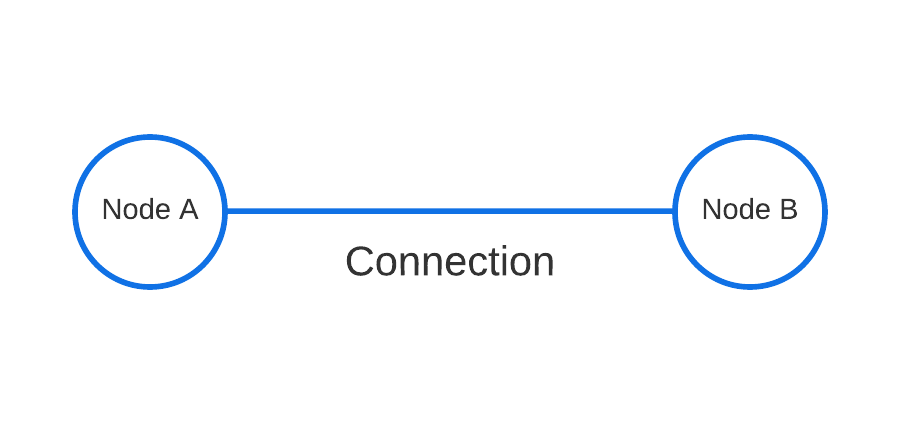
\includegraphics[scale=0.35]{Connection}
	\caption{Visual representation of a simple network graph.}
\end{figure}

\subsubsection{Client}
Client represents a network node that has one to one relationship with the server. Client node never directly communicates with any other client nodes, only with the server. Client exposes a simple API\footnote{https://en.wikipedia.org/wiki/API} for connecting to the server, sending packets and disconnecting from the server.

\begin{table}[H]
	\centering
	\begin{tabular}{|c|c|}
		\hline
		\textbf{Method} & \textbf{Description}                                                                                            \\ \hline
		Connect         & \begin{tabular}[c]{@{}c@{}}Attempts to establish a\\ connection with the server.\end{tabular}                   \\ \hline
		Send            & Sends a packet to the server.                                                                                   \\ \hline
		Disconnect      & \begin{tabular}[c]{@{}c@{}}Disconnects from the server and\\ stops listening for incoming packets.\end{tabular} \\ \hline
	\end{tabular}
	\caption{Client API.}
	\label{table:client-api}
\end{table}

Client also raises important events that occurred during runtime\footnote{https://en.wikipedia.org/wiki/Runtime\_(program\_lifecycle\_phase)}, to which many subscribers can listen to.

\begin{table}[H]
	\centering
	\begin{tabular}{|c|c|}
		\hline
		\textbf{Event} & \textbf{Description}                                                                                                              \\ \hline
		Connecting     & \begin{tabular}[c]{@{}c@{}}Invoked each time client starts the process of\\ establishing connection with the server.\end{tabular} \\ \hline
		Connected      & \begin{tabular}[c]{@{}c@{}}Invoked each time client\\ successfully connects to the server.\end{tabular}                           \\ \hline
		ConnectFailed  & \begin{tabular}[c]{@{}c@{}}Invoked each time client fails to\\ establish a connection with the server.\end{tabular}               \\ \hline
		PacketReceived & \begin{tabular}[c]{@{}c@{}}Invoked each time a data-packet\\ is received from the server.\end{tabular}                            \\ \hline
		Disconnected   & \begin{tabular}[c]{@{}c@{}}Invoked each time client\\ disconnects from the server.\end{tabular}                                   \\ \hline
	\end{tabular}
	\caption{All of the possible events that can be raised by a client node.}
	\label{table:client-events}
\end{table}

\subsubsection{Server}
Server represents a network node that has one to many relationship with clients. Server node never communicates with any other server nodes. Server exposes a simple API for starting the server, sending packets to one or more clients, kicking specific clients and stopping the server.

\begin{table}[H]
	\centering
	\begin{tabular}{|c|c|}
		\hline
		\textbf{Method} & \textbf{Description}                                                                                         \\ \hline
		Start           & Starts listening for incoming client packets.                                                                \\ \hline
		SendToOne       & Sends a packet to one specific client.                                                                       \\ \hline
		SendToMany      & Sends a packet to many clients.                                                                              \\ \hline
		SendToAll       & Sends a packet to all connected clients.                                                                     \\ \hline
		Kick            & Deliberately disconnects specific client.                                                                    \\ \hline
		Stop            & \begin{tabular}[c]{@{}c@{}}Disconnects all clients and prevents\\ any further incoming packets.\end{tabular} \\ \hline
	\end{tabular}
	\caption{Server API.}
	\label{table:server-api}
\end{table}

Server also raises important events that occurred during runtime, to which many subscribers can listen to.

\begin{table}[H]
	\centering
	\begin{tabular}{|c|c|}
		\hline
		\textbf{Event}     & \textbf{Description}                                                                                                   \\ \hline
		Started            & \begin{tabular}[c]{@{}c@{}}Invoked each time server starts and\\ begins listening for client connections.\end{tabular} \\ \hline
		ClientConnected    & \begin{tabular}[c]{@{}c@{}}Invoked each time a new client\\ connects to the server.\end{tabular}                       \\ \hline
		ClientDisconnected & \begin{tabular}[c]{@{}c@{}}Invoked each time an already connected\\ client disconnects from the server.\end{tabular}   \\ \hline
		PacketReceived     & \begin{tabular}[c]{@{}c@{}}Invoked each time a data-packet\\ is received from a client.\end{tabular}                   \\ \hline
		Stopped            & \begin{tabular}[c]{@{}c@{}}Invoked each time server stops and no\\ longer listens for client connections.\end{tabular} \\ \hline
	\end{tabular}
	\caption{All of the possible events that can be raised by a server node.}
	\label{table:server-events}
\end{table}

\subsubsection{Simulation}
When building a networking application using local network, connection is almost always going to be flawless. There will be no packet loss, latency will be minuscule and there will generally be no problems.\\

However, real-life networks are unpredictable; packet-loss will occur and latency is going to vary. In order to test how your application would behave under those real network conditions, optional network simulation can be enabled. It allows each node to specify artificial packet-loss and any amount of latency.


\chapter{High-level library}
This chapter explains in detail the concept and implementation of a high-level library developed for the Unity\footnote{https://unity.com/} game-engine.

\section{Component: Network Manager}

\section{Component: Network Object}

\section{Component: Network Behavior}

\section{Component: Network Transform}
\textit{NetworkTransform} is a concrete implementation of \textit{NetworkBehavior} that solves the problem of synchronizing object's position, rotation and scale.

\begin{figure}[H]
	\centering
	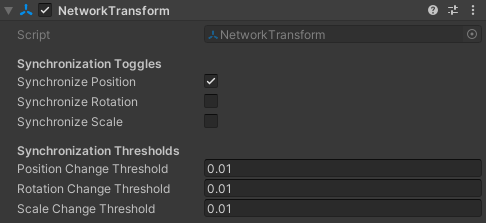
\includegraphics[scale=1.1]{NetworkTransform-inspector}
	\caption{NetworkTransform component displayed inside Unity's inspector.}
\end{figure}

It is a powerful component that allows user to synchronize object's transform by simply attaching the component to it. Since transform synchronization is one of the most commonly encountered problems when creating a networked game, general solution such as this one saves developer a lot of time.\\

However, since transform synchronization is so common, simple ease of use is not enough; it also must be efficient. Component has to be able to support potentially hundreds of simultaneous instances and to achieve that it exploits the following facts:

\begin{enumerate}
	\item Object's rotation or scale is in many cases never-changing. That fact can be exploited to save bandwidth by giving the user ability to disable synchronization of particular transport's component (position, rotation or scale). If a component is disabled, its data is never going to be added to the outgoing synchronization packet, saving valuable bandwidth.
	
	\item If object's transform does not change, it does not need to be synced. Transform is marked as changed only if one of its enabled components' values has been changed by a value greater than threshold defined for that component. if transform is changed, only modified components are included in the sync packet. This way only changed components of changed transforms are synced, massively reducing the number of sync packets required.
\end{enumerate}

\begin{figure}[H]
	\centering
	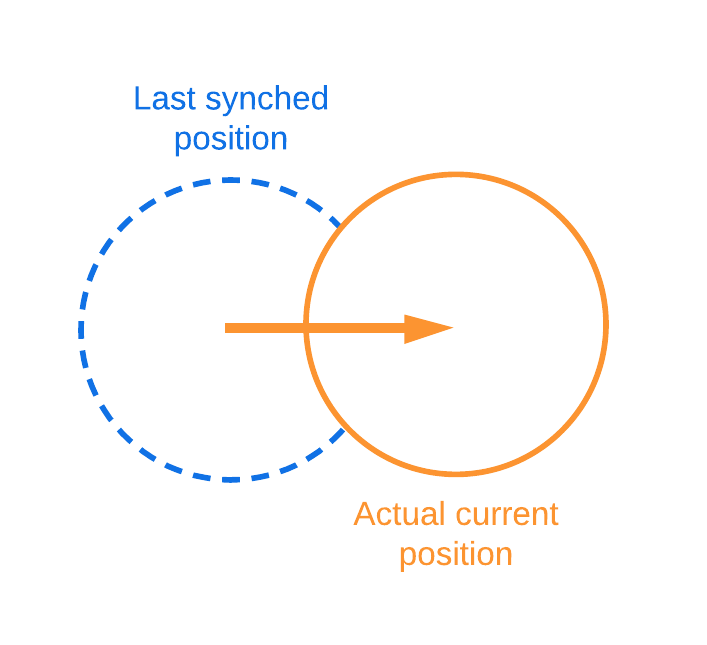
\includegraphics[scale=0.3]{NetworkTransform-position-diagram}
	\caption{Example of position synchronization. Orange arrow is a delta vector that shows the change in position since last synchronization. If length of the delta vector exceeds user-defined threshold, synchronization will occur.}
\end{figure}

\textit{NetworkTransform} is also allowed on nested objects (for example, player's body could have one, but also player's head another, which synchronizes only head rotation). In order to understand how this is achieved, packet structure must be explained.

\begin{figure}[H]
	\centering
	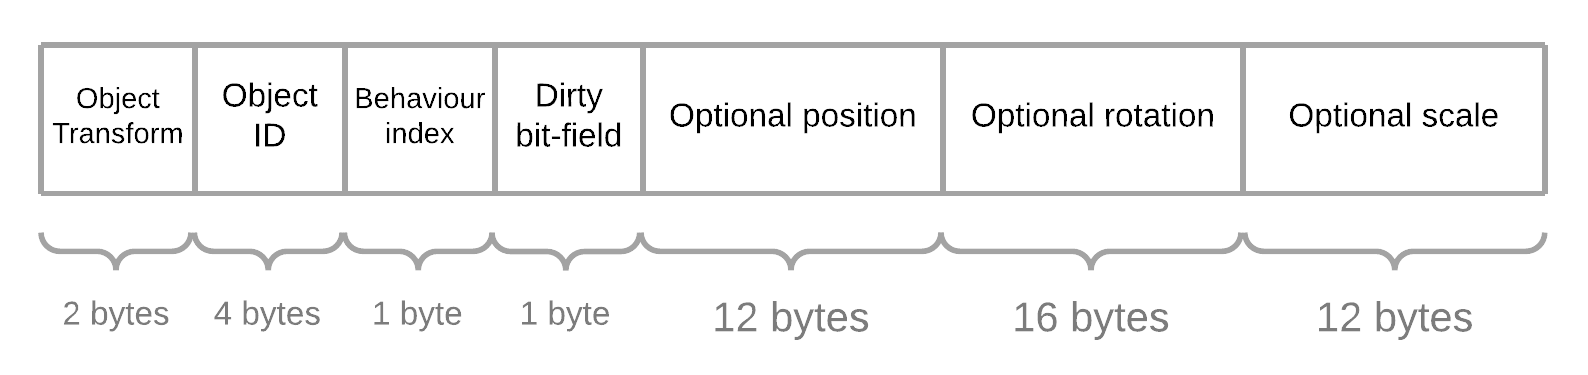
\includegraphics[scale=0.25]{NetworkTransform-packet-structure}
	\caption{Structure of the packet that is sent by the \textit{NetworkTransform} component.}
\end{figure}

Component starts by inserting 2-byte value that indicates that packet contains object transform information. It is followed by specific object's ID that uniquely identifies it, allowing receiver to know which exactly which object's transform should be modified. After that, behavior index is provided to the receiver, which allows the receiver to know which exact child transform should be modified (this information allows for nested networked transforms).\\

To indicate whether a transform's component is included in a packet, so called \textit{dirty bit-field} is used. It is a single byte whose first bit indicates whether position is included in the packet, second bit indicates whether rotation is included and third bit indicates whether scale is included. In the end, actual position, rotation and/or scale of an object is provided.\\

This component uses sequenced channel to send its packets, as only the most recent data is relevant. This system provides user with a very simple, but bandwidth-efficient way to synchronize transform of any networked object. 

\section{Component: Network Spawner}



\chapter{Uvod}
Uvod rada. Nakon uvoda dolaze poglavlja u kojima se obrađuje tema.

\chapter{Zaključak}
Zaključak.

\bibliography{literature}
\bibliographystyle{fer}

\begin{sazetak}
Sažetak na hrvatskom jeziku.

\kljucnerijeci{Ključne riječi, odvojene zarezima.}
\end{sazetak}

\engtitle{Development and application of a videogame multiplayer networking library}
\begin{abstract}
Abstract.

\keywords{Keywords.}
\end{abstract}

\end{document}
